\Chapter{Modern módszerek a nyelvfeldolgozásban}

Az utóbbi idők legjelentősebb fejlődését a területen a neurális hálózatok megjelenése indukálta. Korábban számos próbálkozás született szabályok, sablonok, statisztikai megoldások felhasználásával, azonban ezek például egy chatbot vagy szöveggenerálási feladat esetén hamar problémákba ütköztek, hiszen egy újabb, addig ismeretlen nyelvi elem vagy egy speciálisabb kontextus teljesen meg tudta állítani ezen programok működését. További probléma volt, hogy mivel magát a nyelvet, annak kódolását és dekódolását is emberek találták ki emberi aggyal, így egyszerű képletekkel, szabálybázisokkal ez a probléma nem volt megoldható, mivel az emberi agy - mint az számos kutatásból kiderült - nem használja beépítve ezeket a működéseket, például nem kezdi el egyenként, szekvenciálisan feldolgozni a betűket, hanem belső állapotától függően képes egyben látni szavakat, mondatokat és leginkább predikciókkal dolgozik, mint sem pontosan leírt, kötött műveletekkel, szabályokkal.

\Section{Neurális hálózatok}

Mindezen problémák miatt logikus lépés volt megvizsgálni az emberi agyat és előállni egy olyan koncepcióval, mely képes modellezni az agy mintafelismerési képességét és ezáltal új távlatokat nyitni a nyelvfeldolgozás területén. Ezek voltak a \textbf{neurális hálózatok}.

Az idők során számos neurális hálózat típus jelent meg: perceptron, feed forward, MLP, konvolúciós, visszacsatolt(RNN) stb. Ezek közül számunkra a nyelvfeldolgozás területén a legfontosabb és legtöbbet használt típus az RNN(Recurrent Neural Network).

A neurális hálózatok felépítése nagyon változatos lehet, azonban számos közös jellemzőjük akad. Minden hálózatnak tartalmaznia kell egy bemeneti réteget, egy rejtett réteget és egy kimeneti réteget. Ezen rétegek jellege a feladat típusától függően változtatható, például a hálózat bemenete lehet többdimenziós, a rejtett rétegekben változtathatjuk a neuronok kötéseit, illetve az adatmozgások irányát, a kimenete pedig lehet egy skalár mennyiség vagy egy vektor, attól függően, hogy osztályozni vagy regressziót számítani szeretnénk.

\textbf{RNN} esetén a feladat egy szekvencia feldolgozása, ami lehet egy kép, amit szeretnénk felcímkézni, hangfájlok, amik segítségével beszédet szeretnénk felismerni, illetve akár egy szöveg, amit szeretnénk lefordítani vagy értelmezni. Ami közös ezekben a feladatokban, hogy mindegyik problémakör esetén a feldolgozás során a hálózat bemenete és kimenete jelentősen függ egymástól, vagyis a szekvencia egyes elemeinek értelmezése függ a korábbi elemek értelmezésétől.

\begin{figure}[h]
\centering
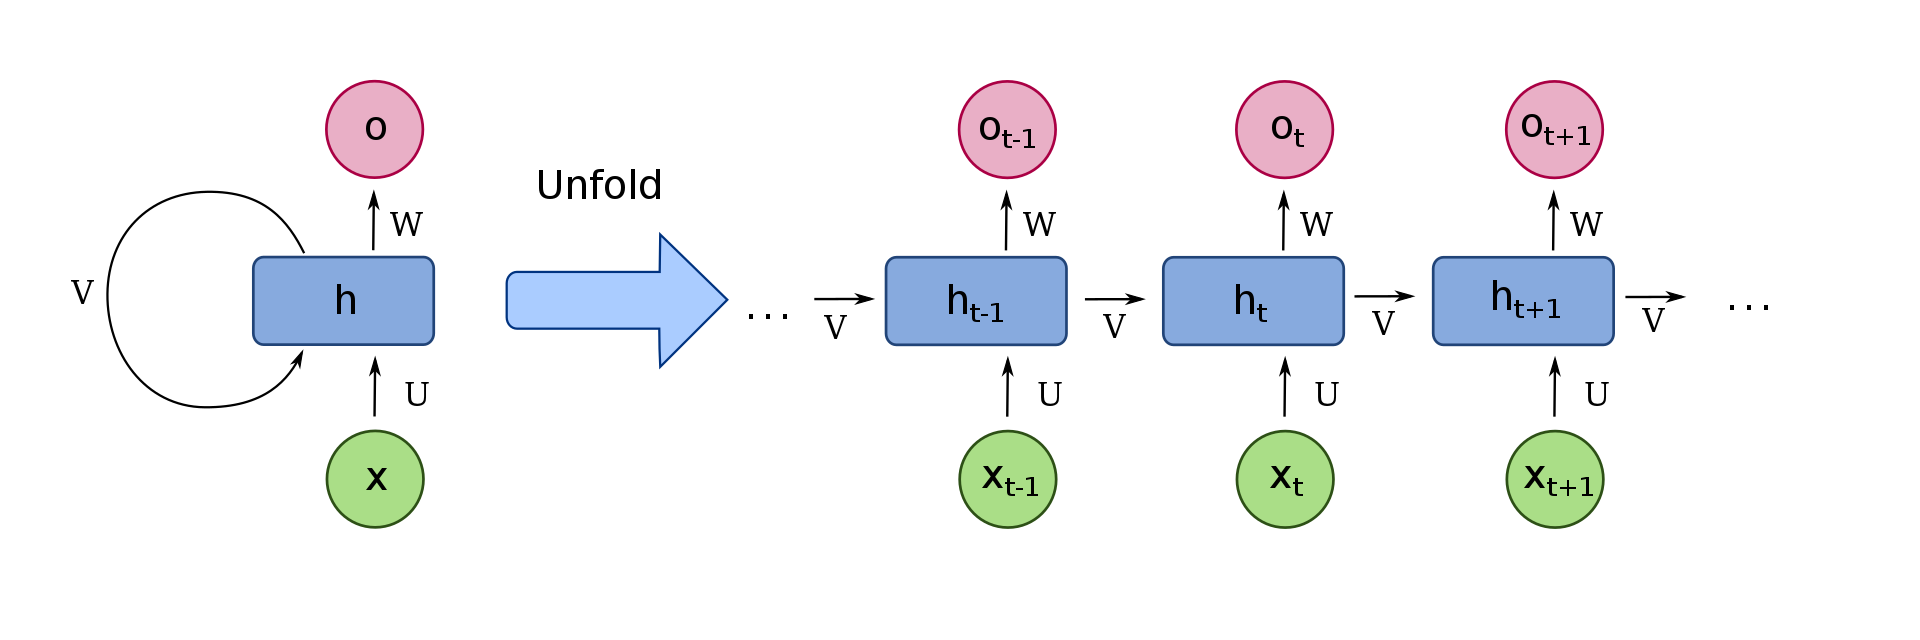
\includegraphics[scale=0.2]{images/rnn.png}
\caption{Az RNN működése \cite{rnn}.}
\label{fig:rnn}
\end{figure}

Kiváló példa erre a szövegfordítás, hiszen a fordítás során fontos a szavak rendje, tehát a hálózatnak sorban, egymás után kell vennie a forrásszöveg szavait és kimenetén ezen szavak adott nyelvű megfelelőjének kell megjelennie.

Ez a működés jelentős előrelépés volt, azonban számos probléma felmerült ennek kapcsán. Az egyik ilyen probléma a hosszabb szövegek értelmezése volt. Ilyenkor a hálózat egyszerűen elfelejtette azt a tudást, amit a szöveg értelmezésének elején megszerzett, ezt hívjuk “vanishing gradients” problémának. Ennek magyarázata a hibafüggvény gradiensében keresendő, ami nem más, mint a hibafüggvény deriváltja a hibagörbe mentén. Amikor ez a gradiens túl kicsi, akkor idővel még kisebbé válik és ezekkel az alacsony, nagyon 0-hoz közeli értékkellel kezdi el frissíteni a hálózat súlyait, egészen addig, amíg azok le nem nullázódnak. Ebben az esetben a hálózat nem tanul tovább. Ennek a problémának létezik a fordítottja is, az “exploding gradients”, melynek során a gradiens túl nagy lesz, ezáltal egy instabil modellt alkotva, melynek hatására a súlyok túl nagyok és idővel NaN értékűek lesznek.

Ezen problémákra születtek megoldások, például a hálózat komplexitásának csökkentése, vagyis a rejtett rétegek számának redukálása, azonban ez nem mindig vezet optimális megoldásra.

Egy másik probléma az RNN-el, hogy a hálózat szekvenciális feldolgozásra készült mivoltából adódóan egyszerűen nem jól párhuzamosítható, vagyis a mai modern hardverekkel, például egy rengeteg, erőteljes párhuzamosításra használható maggal felszerelt GPU-n nem tudjuk effektíven tanítani a hálózatot, ami a nagyobb szövegek értelmezését rettentően időigényessé teszi.

\Section{Transformer hálózatok}

Az RNN tehát minden problémájának ellenére is hatalmas sikereket ért el az NLP területén, azonban 2017-ben egy új neurális hálózat típus jelent meg:\\
az átalakító(transformer), ami a fentebb említett problémákat javítva és a fejlesztést is egyszerűbbé téve átvette a vezetést a szövegfeldolgozás területén.

Az átalakítókat a Google és a Torontói Egyetem szakemberei fejlesztették ki 2017-ben és meg is jelentettek egy cikket "Attention Is All You Need"\cite{attention} címmel, amiben részletezték ezen átalakítók működését. Talán a legnagyobb újítás a párhuzamosíthatóság területén jelent meg, mivel ezeket a hálózatokat a megfelelő eszközökkel hatalmas mennyiségű adatokkal lehet tanítani. Például a Google T5 nevű átalakító modelljének a többnyelvű változatát a c4/multilingual nevű adathalmazzal tanították, ami 26.76 TiB méretű(1 TiB = 1.1 TB). Később az OpenAI vállalat GPT-3 nevű modellje még ezt is túlszárnyalta szinte a teljes publikus internetet tartalmazó 45 TB méretű szöveges adatot tartalmazó tanítóadatával. Ezen méretű tanítóhalmaz korábban elképzelhetetlen volt az RNN-ek használatával.\\
Az átalakítók működését 3 fontos fejlesztésre lehet lebontani:

\begin{itemize}
\item Pozíciókódolások(Positional Encodings)
\item Figyelem(Attention)
\item Önfigyelem(Self-Attention)
\end{itemize}

A \textbf{pozíciókódolással} a korábbi RNN-ek szekvencialitását oldották fel azáltal, hogy a mondatokat nem a szavak sorrendjében kezdték el feldolgozni, hanem a mondat minden szavát ellátták egy annak mondatban elfoglalt pozícióját jelentő címkével. Ez a struktúra szó-sorszám párokat jelent, amiket a hálózat megtanul hatásosan használni. Ennek segítségével a szavak sorrendje immáron nem a hálózat struktúráját jelenti, vagyis a szekvencialitást, hanem egyszerű feature-nek, adatnak tekinthető.

A \textbf{figyelem} egy olyan mechanizmus, melynek segítségével a modell végigmehet a bemenet minden szaván és megadhatja egy szónak a jelentését az alapján, hogy melyik ismert idegennyelvű szóhóz áll a legközelebb a szintaktikája. Ezt a tudást a tanítás során szerzi meg a modell, ezért is van szükség minnél nagyobb adathalmazokra. Ez a működés elsősorban a modell célterületén vagyis  szövegfordítások esetén hasznos, ahol egy adott nyelvű mondat fordításánál a szórend változhat, és nem elég szimplán az egyes szavakat lefordítani, hanem szükség van egyfajta háttértudásra, nyelvi ismeretekre a fordítás során. Pélául a \textit{"The agreement on the European Economic Area was signed in August 1992."} angol nyelvű mondat francia fordítása \textit{"L'accord sur la zone économique européenne a été signé en août 1992."} Láthatjuk, hogy a \textit{"European Economic Area"} fordítása \textit{"la zone économique européenne"}, tehát a szórend és a szavak alakja is változik. Ebben az esetben nem elég az egyes szavakat szekvenciálisan fordítani, hanem minden angol szóhoz a forrásmondatban fel kell építeni egyfajta hőtérképet a francia fordításokkal és a modellnek végig kell néznie az egyes szavakat és meg kell mondania, hogy melyik angol szóhoz melyik francia szó illeszkedik. Esetünkben például az \textit{"European"} szóhoz illeszkedik az \textit{"européenne"} és az \textit{"économique"} szó is, azonban a modell korábbi tanításából adódóan tudja, hogy itt az \textit{"européenne"} fordítás lesz a helyes.

\begin{figure}[h]
\centering
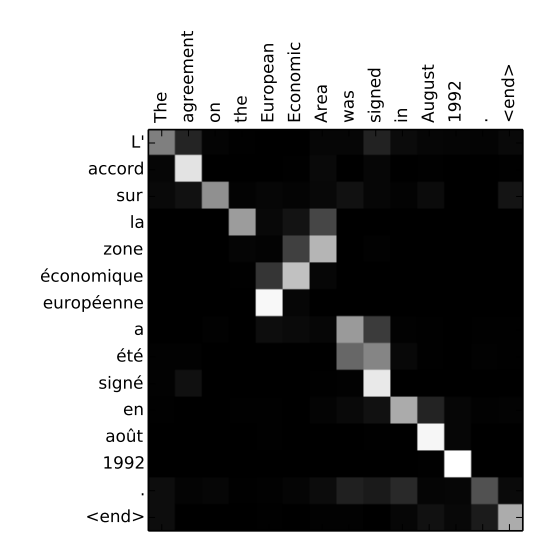
\includegraphics[scale=0.9]{images/translate_heatmap.png}
\caption{Angol-francia fordítás hőtérképe \cite{translation}.}
\label{fig:translate_heatmap}
\end{figure}

Az utolsó fontosabb fejlesztés az \textbf{önfigyelem}, ami talán a legfontosabb a szövegértelmezés szempontjából. Korábban láthattuk, hogy a figyelem segítségével a modell képes megfelelő sorrenben fordítani a szavakat, azonban ez még nem elég ahhoz, hogy képes legyen érteni is az egyes szavak jelentését és ezáltal más szövegfeldolgozási feladatokat is meg tudjon oldani. Ennek érdekében szükségessé vált, hogy a modell mögött álló neurális hálózat felépítsen egy belső reprezentációt az adott nyelvről. Ez a belső működés leginkább a különböző képfelismerési hálózatok(CNN) rétegeihez hasonló, ahol az egyes régetek képesek felismerni éleket, alakzatok és egyéb magasabb szintű, komplexebb struktúrákat, mint emberek, állatok vagy tárgyak. Nyelvi környezetben ezen rétegek képesek felismerni a különböző nyelvtani szabályokat, szinonímákat és szövegrészleteket. A célja ezen rétegeknek, hogy minnél jobban megtanulják az egyes nyelvtani elemeket és kontextusokat, így a modell képes lesz szinte bármilyen nyelvi feladatot megoldani.\\
Vegyük példának a következő angol nyelvű mondatokat:

\begin{enumerate}
\item \textit{"Server, can I have the check?"}
\item \textit{"Looks like I just crashed the server."}
\end{enumerate}

A \textit{"server"} szó ebben a 2 mondatban 2 különböző jelentéssel bír: az egyik mint felszolgáló vagy pincér, míg a másik egy webes kiszolgálóra utal. Mi emberek a \textit{"server"} szó körül lévő szavakból könnyen meg tudjuk különböztetni a 2 jelentést, azonban ez a gépeknek korábban nem volt egyszerű feladat. Az önfigyelem erre a feladatra nyújt megoldást azáltal, hogy képes az egyes szavakat más szavakhoz kötni és így a modell megtanulja, hogy abban az adott kontextusban mit is jelenthet az a szó. Például az 1. mondatban a \textit{"server"} szó mellett megtalálható a \textit{"check"}, a \textit{"can"} és a \textit{"have"} szó is, melyek együtt sűrűbben szerepelnek egy éttermi szituációt leíró kontextusban, mint a webfejlesztés esetében, tehát itt egy pincért jelent a szó, míg a 2. mondatban megtalálható a \textit{"crashed"} szó, ami pedig az informatikában és webes környezetekben gyakoribb, ezáltal a \textit{"server"} itt egy webkiszolgálót jelent.

\begin{figure}[h]
\centering
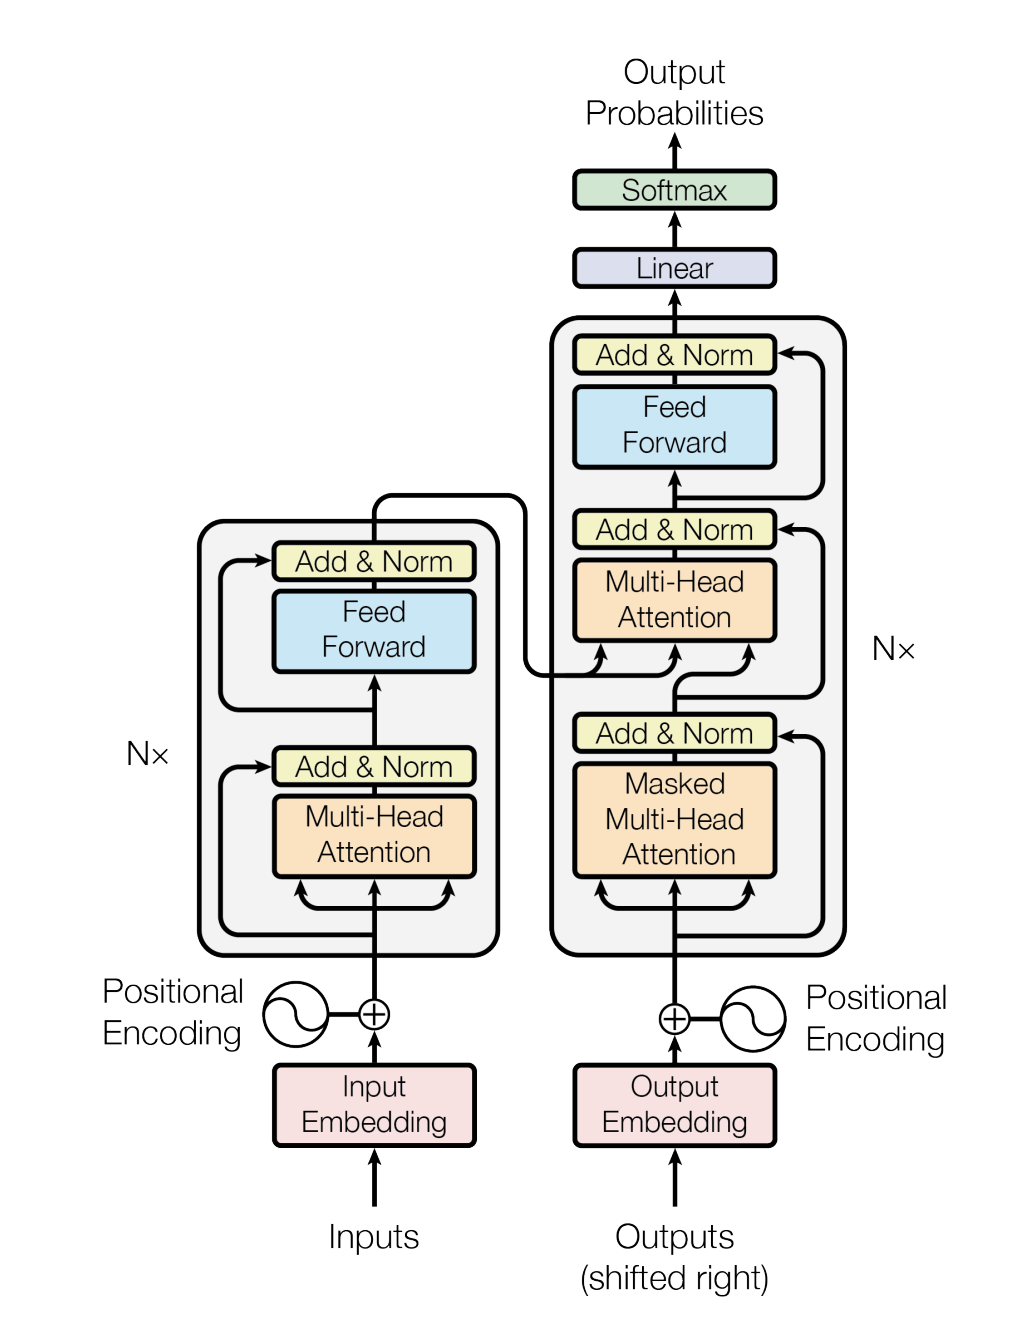
\includegraphics[scale=0.4]{images/transformer.png}
\caption{Az átalakító modell architektúrája  \cite{attention}.}
\label{fig:transformer}
\end{figure}

\Section{A BERT modell}

Ez a 3 fontosabb fejlesztés indítottal el útjára az átalakító alapú modelleket, melyek közül az első jelentősebb a Google által 2018-ban kifejlesztett \textbf{Bidirectional Encoder Representations from Transformers(BERT)} volt. A BERT nem csak egy újfajta modell architektúra volt, hanem egy teljesen új betanított modell, amit ingyenesen letölthetővé is tettek. Kisebb átalakításokkal számos probléma megoldására képes volt: szövegösszefoglalás, kérdés-válasz generálás, osztályozás és még sok más feladat. Működésének legfontosabb fejlesztése az átalakító modell kétirányú kiterjesztése volt. Korábban az átalakító modellek a tanítás során balról jobbra vagy kombináltan balról jobbra és jobbról balra dolgozták fel a szövegeket. Ezzel szemben a BERT a szavak értelmezésénél a környező szavakat mind a két lehetséges irányban egyszerre dolgozza fel, ami a szövegek mélyebb megértését teszi lehetővé.\\
Ahhoz, hogy ez a működés megvalósuljon 2 fajta tanítási stratégiát használ a BERT:

\begin{itemize}
\item Masked-Language Modeling (MLM)
\item Next Sentence Prediction (NSP)
\end{itemize}

A \textbf{Masked-Language Modeling} az adott szöveg, pontosabban a szöveg szavainak mélyebb megértését célozza. A BERT hálózat tanítása során az egyes mondatok szavainak kb. 15\%-át kicserélik [MASK] tokenekre. Ezt követően a modell megpróbálja kitalálni ezeket a maszkolt szavakat a körülötte lévő nem maszkolt szavak kontextusa alapján. A predikció során a maszkolt szavak mindkét oldaláról figyelembe veszi a nem maszkolt szavak kontextusát, innen ered a kétirányúsága a modellnek. Ez a működés nagyon hasonlít ahhoz, ahogy mi emberek értelmezünk egy szöveget vagy próbáljuk kitalálni egy ilyen feladat során a hiányzó szavakat.

\begin{figure}[h]
\centering
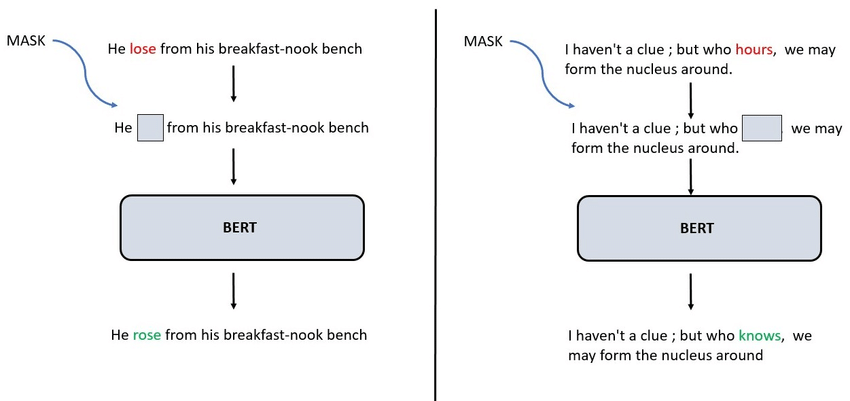
\includegraphics[scale=0.4]{images/bert_mask.png}
\caption{Maszkolt szavak beillesztése a BERT működése során \cite{bert}.}
\label{fig:bert}
\end{figure}

A \textbf{Next Sentence Prediction} esetén az MLM-el szemben nem a szöveg szavainak a megértése a cél, hanem az egyes mondatok közötti kapcsolatok feltárása. Ennek érdekében a tanítás során a modell mondat párokat kap, melyek második eleméről el kell döntenie, hogy az első mondat után következnek-e az eredeti forrásszövegben. A gyakorlatban a bemeneti szöveg mondatainak 50\%-a olyan páros, ahol a mondatok egymás után következnek, a másik 50\%-a pedig olyan, ahol a második mondat random kerül kiválasztásra és feltesszük, hogy a random mondat nem lesz kapcsolatban az első mondattal.

\begin{figure}[h]
\centering
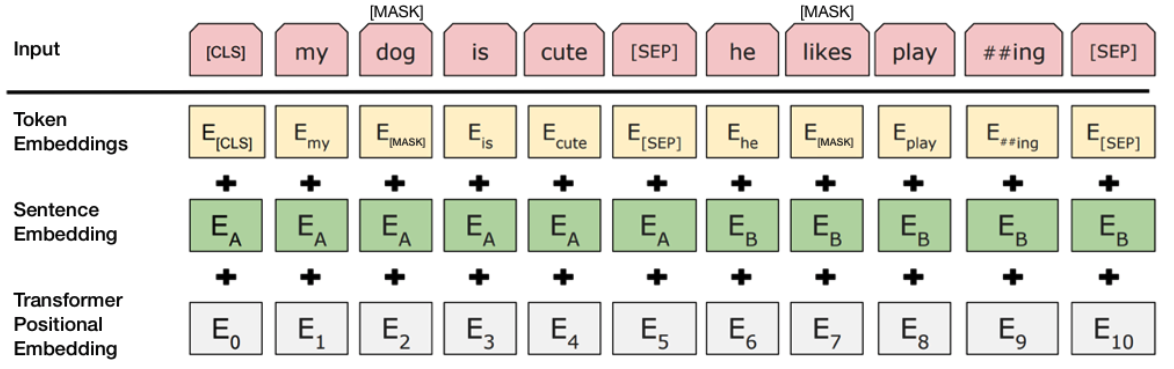
\includegraphics[scale=0.3]{images/next_sentence_prediction.png}
\caption{Next Sentence Prediction a gyakorlatban \cite{bert2}.}
\label{fig:bert2}
\end{figure}

\Section{A T5 modell}

A BERT jelentős sikerei után elkezdődtek a kutatások a modell felhasználók számára való egyszerűsítésére, adathalmazának kibővítésére és tisztítására, illetve a modell képességeinek újabb feladatokra történő kiterjesztésére. 2020-ban a Google kutatói elő is álltak a \textbf{T5} nevezetű modellel. A modell fő célja az volt, hogy a korábbi fejlesztésekkel ellentétben a modell bemeneti forrásszövege és a kimenet is egységes szöveg formátumú legyen minden NLP feladat esetén.

A modell előtanítása során a Colossal \textbf{Clean Crawled Corpus(C4)} nevű adathalmazt használták, ami közel 700 GB méretű és a  Common Crawl adathalmaz egy tisztított verziója. A C4 adathalmaznak létezik többnyelvű változata is az \textbf{mC4}, amely már tartalmazza a magyar nyelvet is sok más nyelv mellett. Az mC4 adathalmazon tanított T5 pedig az \textbf{mT5} nevet viseli és képes magyar nyelvű szövegek generálására is.

Belső működésében a T5 hasonlóan működik mint a BERT. A Masked-Language Modeling ugyanúgy megmaradt, azonban kibővítették azzal, hogy immáron nem csak egy-egy szót, hanem egyszerre több egymás melletti szót is maszkol, amit a modellnek ugyanúgy ki kell majd találnia. Ennek érdekében a forrásszöveget bemenet-cél párosokra bontja és ezeket fogja megtanulni a tanítás során. A BERT-el ellentétben itt a kimenet nem egyetlen szó lesz, hanem egy generált szöveg, tetszőleges mérettel.

\newpage

\begin{figure}[h]
\centering
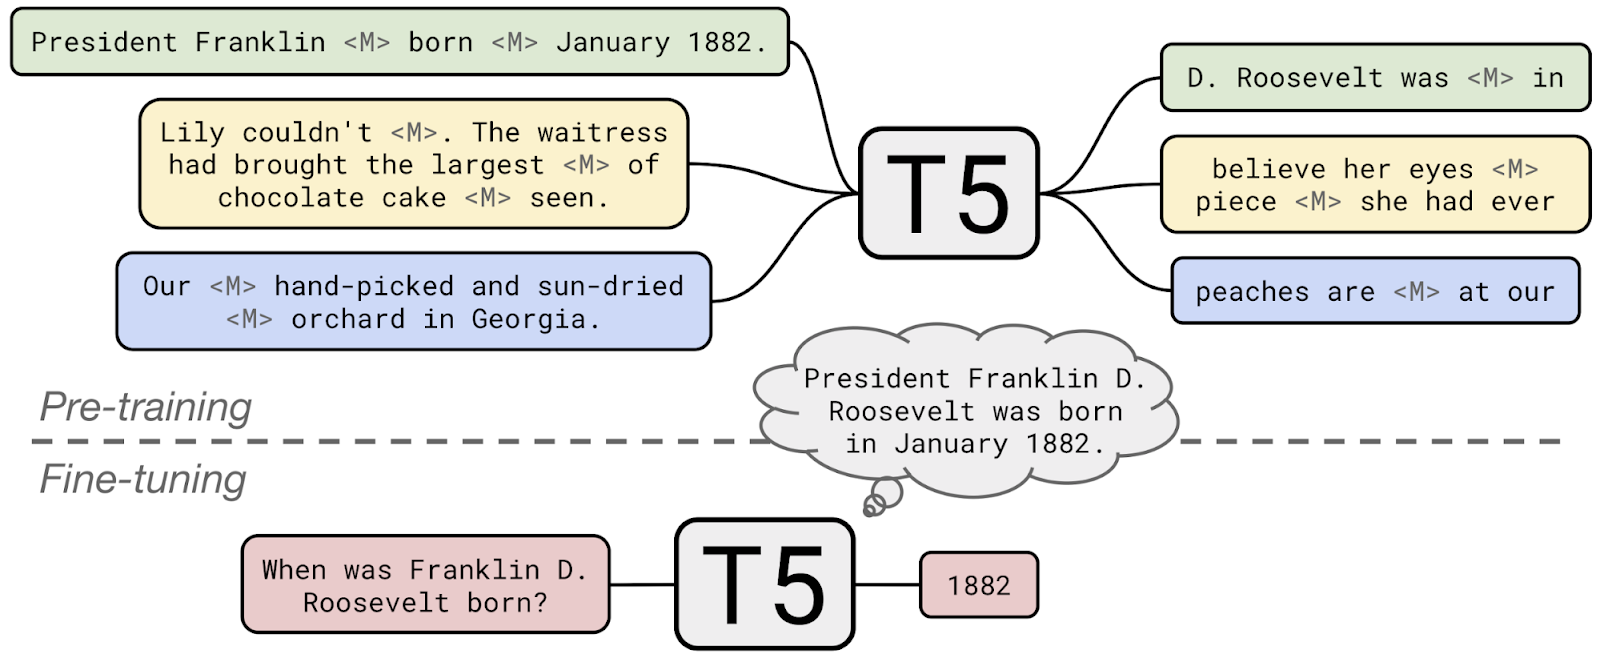
\includegraphics[scale=0.2]{images/t5.png}
\caption{T5 modell a tanítás előtt és után \cite{t5}.}
\label{fig:t5}
\end{figure}

Az előtanítás után a modellt finomhangolták számos NLP feladatra: fordítás,\\
összegzés, mondathasonlóság stb. A finomhangolás során bevezettek egy egyedi formátumot a különböző feladatok különválasztására. A forrásszöveg elé beszúrtak egy prefixet, ami az adott NLP feladatot jelöli. Ennek formátuma:

\textbf{feladat\_ azonosítója: forrászöveg}

Ez azért volt szükséges, hogy a modell súlyait feladatok szerint tudják csoportosítani és így az egyes feladatokra való finomhangolás nem zavar bele a többi feladat megoldásába.

\Section{A GPT-3 modell}